\section{Tests for CI} Providing a set of regression tests for the CI pipeline is clearly a good practice, since they will be executed with every change provided to the remote repository and make sure that if any of those changes will affect the functionality of the tested code the pipeline will fail and the code with defects will not be deployed. Moreover, tests will tell the developer exactly what unit was affected by their changes and require a fix.


%https://vitest.dev
\subsection{Vitest} Vite is a frontend build tool used for the BI-DBS frontend. Vitest is a unit test framework built on top of Vite. It is a suitable tool for implementing tests in the project like the BI-DBS frontend which uses Vite. Vitest cares a lot about performance and speed, which makes it a good choice for tests that will be a part of CI pipeline.

\subsection{Tests} The authorization module is composed of four main services which I have implemented for authentication and authorization processes including additional features like a refreshing of token and logging out and others. Therefore I have created unit tests for the functionalities of those services.\\

\noindent \textbf{Services and what functionalities they provide:}

\begin{itemize}
    \item \emph{Generating the access token service.} The process of getting the access token enables the application to log in the user on the frontend after an authorization server has successfully authorized the user and provided the client with the authorization code. This service is focused on exchanging that code for an access token with the backend and handling the response from the server.
    \item \emph{Refreshing the access token service.} Refreshing process prolongs the authorized status for a user without the need of submitting credentials, which is implemented by exchanging the refresh token and current access token for the new access token with the backend. 
    \item \emph{Rejecting the access token.} The process of logging out is implemented as a rejection of a token which includes removing all of the user's data from the user's store along with permissions to access the components which require authorization.
    \item \emph{Authorization service.} The services described above also need some additional functionalities like parsing the data from the request and preparing the URL for communication with the authorization server which are implemented in the authorization service. 
\end{itemize}


% \paragraph*{Test cases for the authorization service} 
% \begin{itemize}
%     \item Test for checking the correct creation of the complex URL for sending the request for to the authorization service to initiate the authorization process.
%     \item Test for controlling parsing the access token into a user's identity information and setting the authorized status for the admin role included.
%     \item Test for controlling parsing the access token into a user's profile and setting the authorized status for the guarantor role. 
%     \item Test for controlling parsing the access token into a user's profile and setting the authorized status for the teacher role.
%     \item Test for controlling parsing the access token into a user's profile and setting the authorized status for the student role.
% \end{itemize}


\paragraph*{Test cases for the token generating service} 
\begin{itemize}
    \item \emph{Positive scenario:} 
        \begin{itemize}
            \item \emph{Conditions:} A valid token is successfully returned in the valid response.
            \item \emph{Expected result:} User was successfully authorized.
        \end{itemize}
    \item \emph{Negative scenario} 
        \begin{itemize}
            \item \emph{Conditions:} An invalid token is successfully returned in the valid response.
            \item \emph{Expected result.} The errors from parsing the token are successfully handled and the user was not authorized.
        \end{itemize}
    \item \emph{Negative scenario.} 
        \begin{itemize}
            \item \emph{Conditions:} The request for an access token fails.
            \item \emph{Expected result:} The errors from the request are successfully handled and the user was not authorized.
        \end{itemize}
    
    % A valid token is successfully returned in the valid response. The test is checking the successful login.
    % \item \emph{Negative scenario.} An incorrect token is successfully returned in the valid response. The test is controlling the handling of the error while parsing the token and controls that a user was not logged in.
    % \item \emph{Negative scenario.} The request for an access token fails. The test controls the handling of the error and ensures that a user was not granted any access to the application.
\end{itemize}

\paragraph*{Test cases for the token refreshing service} 
\begin{itemize}
    \item \emph{Positive scenario.} A valid token is successfully returned in the valid response. The test is checking the successful login.
    \item \emph{Negative scenario.} An incorrect token is successfully returned in the valid response. The test is controlling the handling of the error while parsing the token and controls that a user was not logged in.
    \item \emph{Negative scenario.} An incorrect token is successfully returned in the valid response. The test is controlling the handling of the error while parsing the token and controls that a user was not logged in.
\end{itemize}

\paragraph*{Test cases for the token generating service} 
\begin{itemize}
    \item \emph{Positive scenario.} A valid token is successfully returned in the valid response. The test is checking the successful login.
    \item \emph{Negative scenario.} An incorrect token is successfully returned in the valid response. The test is controlling the handling of the error while parsing the token and controls that a user was not logged in.
\end{itemize}


\paragraph*{Test cases for the token refreshing service} 

\paragraph*{Test cases for the token rejecting service} 


\begin{figure}[h]
\centering
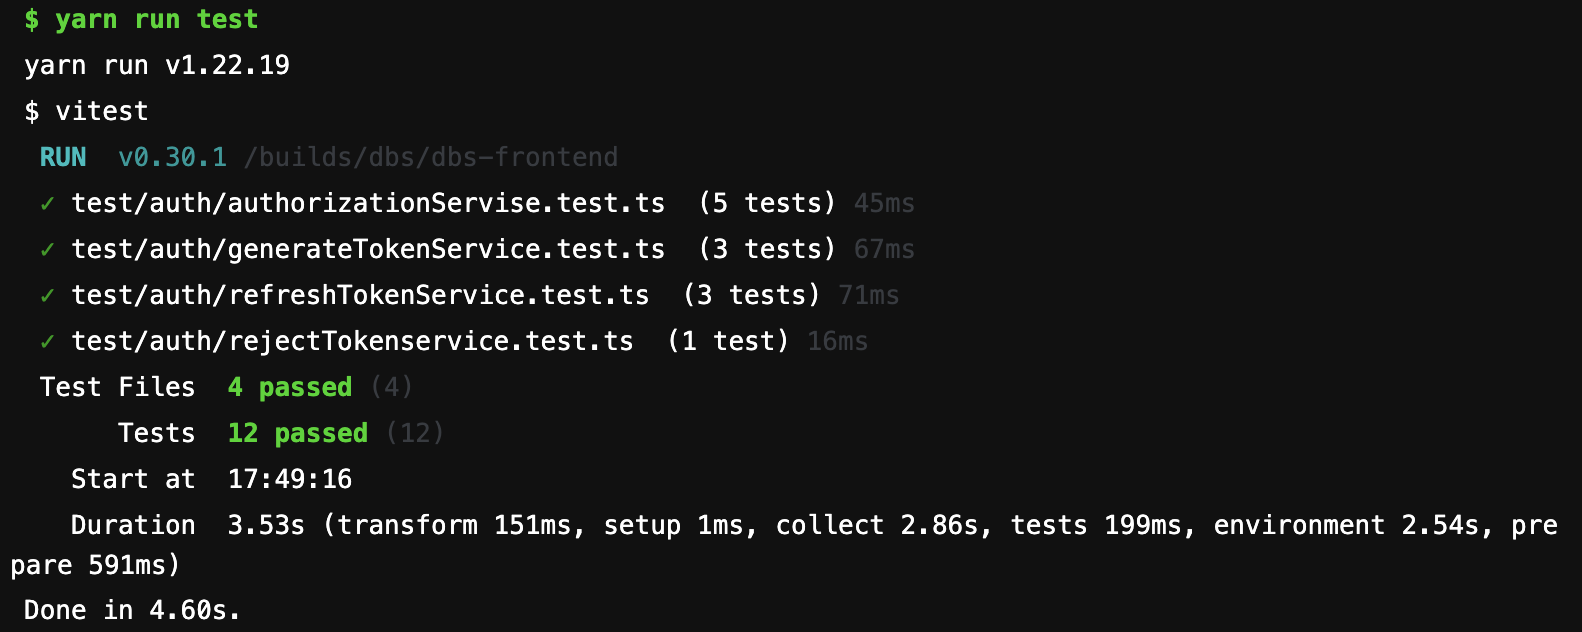
\includegraphics[scale=0.475]{../png/tests.png}
\caption{CI tests}\label{picture:tests}
\end{figure}

vitest unit tests
